% figures/channel-structure.tex
% Standalone TikZ: channel structure — direct, one-level, and two-level channel chains (ch.10).
\documentclass[tikz,border=6pt]{standalone}
\usepackage{tikz}
\usetikzlibrary{arrows.meta,positioning,calc}

\definecolor{vcblue}{HTML}{1A5276}
\definecolor{vcteal}{HTML}{0E6655}
\definecolor{vcgrey}{HTML}{5D6D7E}

\begin{document}
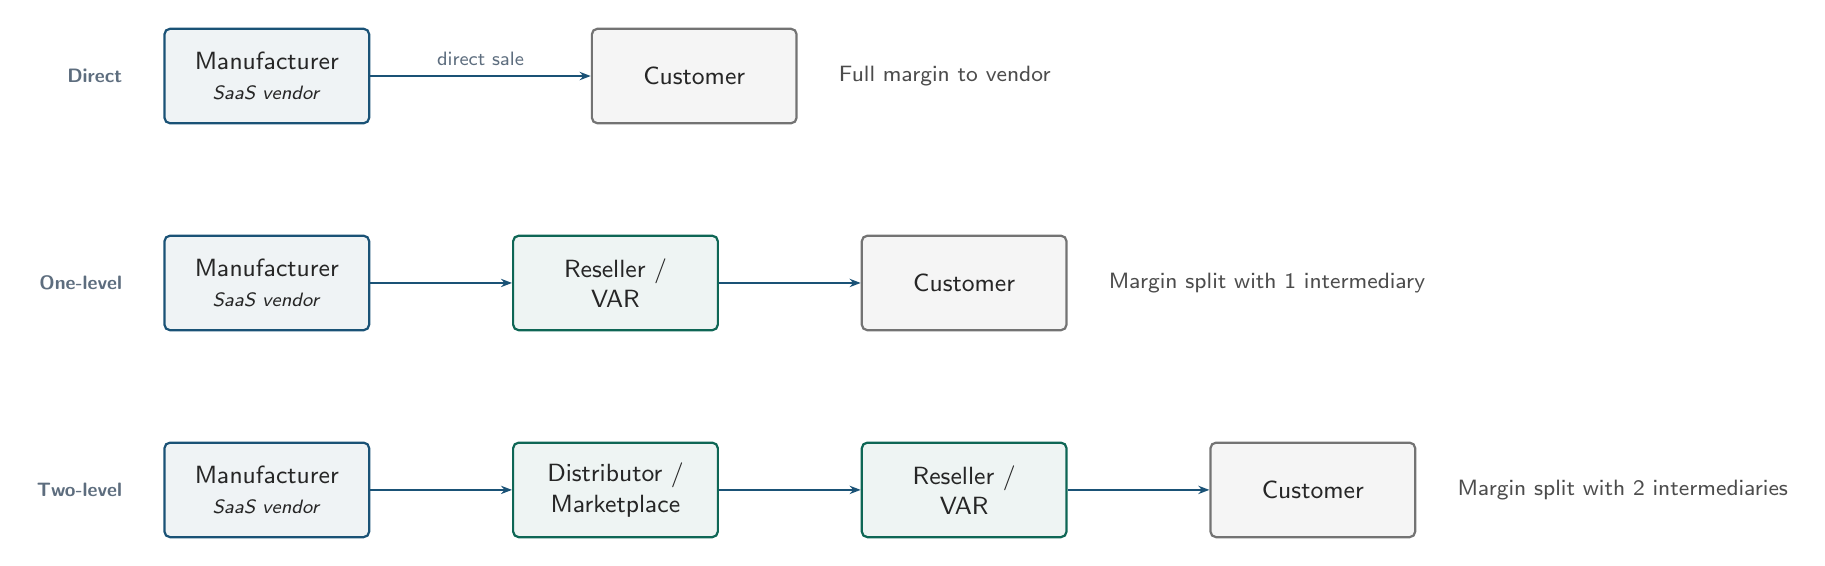
\begin{tikzpicture}[
  node distance=6mm,
  box/.style={draw=vcblue, line width=0.8pt, rounded corners=2pt, fill=vcblue!7,
              font=\sffamily\small, align=center,
              minimum width=26mm, minimum height=12mm, text=black!85},
  interm/.style={draw=vcteal, line width=0.8pt, rounded corners=2pt, fill=vcteal!7,
                 font=\sffamily\small, align=center,
                 minimum width=26mm, minimum height=12mm, text=black!85},
  cust/.style={draw=black!55, line width=0.8pt, rounded corners=2pt, fill=black!4,
               font=\sffamily\small, align=center,
               minimum width=26mm, minimum height=12mm, text=black!85},
  arrow/.style={-{Stealth[length=4pt]}, vcblue, line width=0.9pt},
  lbl/.style={font=\sffamily\scriptsize\bfseries, text=vcgrey, align=left},
  row/.style={font=\sffamily\footnotesize, text=black!70, align=left},
]

%% ---- Row 1: direct channel ----
\node[box]  (m1) {Manufacturer\\{\scriptsize\textit{SaaS vendor}}};
\node[cust, right=28mm of m1] (c1) {Customer};

\draw[arrow] (m1.east) -- node[above,font=\sffamily\scriptsize,text=vcgrey]{direct sale} (c1.west);

%% ---- Row 2: one-level channel ----
\node[box,  below=14mm of m1]  (m2) {Manufacturer\\{\scriptsize\textit{SaaS vendor}}};
\node[interm, right=18mm of m2] (r2) {Reseller /\\VAR};
\node[cust, right=18mm of r2]  (c2) {Customer};

\draw[arrow] (m2.east) -- (r2.west);
\draw[arrow] (r2.east) -- (c2.west);

%% ---- Row 3: two-level channel ----
\node[box,  below=14mm of m2]  (m3) {Manufacturer\\{\scriptsize\textit{SaaS vendor}}};
\node[interm, right=18mm of m3] (d3) {Distributor /\\Marketplace};
\node[interm, right=18mm of d3] (r3) {Reseller /\\VAR};
\node[cust, right=18mm of r3]  (c3) {Customer};

\draw[arrow] (m3.east) -- (d3.west);
\draw[arrow] (d3.east) -- (r3.west);
\draw[arrow] (r3.east) -- (c3.west);

%% ---- Row labels on left margin ----
\node[lbl, left=4mm of m1] {Direct};
\node[lbl, left=4mm of m2] {One-level};
\node[lbl, left=4mm of m3] {Two-level};

%% ---- Margin annotations (right of customer nodes) ----
\node[row, right=4mm of c1] {Full margin to vendor};
\node[row, right=4mm of c2] {Margin split with 1 intermediary};
\node[row, right=4mm of c3] {Margin split with 2 intermediaries};

\end{tikzpicture}
\end{document}
